\section{Reglerschaltung für positive Spannungsversorgung}
\subsection{Aufgabenstellung}
In die Anschlussklemmen des gestellten Experimentierboards ist sowohl ein LM2940 als auch ein LM7805 einzubauen. Als Last soll ein Strom von 1A bei 5V fließen dazu ist ein $R_{Last}$ zu dimensionieren. 

Von dieser Schaltung sind folgende Werte zu messen:
\begin{itemize}
    \item Spannungsrippel, Eingangsspannung an $C_1$ bei $C_1=4700\mu \text{F}$ und $C_1=1000\mu \text{F}$ und Ausgangsspannung.
    \item Minimal mögliche Eingangsspannung für den LM2940 und den LM7805.
    \item der Wirkungsgrad der beiden Regler.
\end{itemize}
\subsection{Dimensionierung}
Es soll bei einer Ausgnagsspannung von $V_{out} = 5V$ ein Strom von $I=1\rm A$ fließen. Der Widerstand R ist danach zu dimensionieren.
\begin{align}
    R&= \frac{U}{I} = \frac{5}{1} = 5\Omega \\
    P_{Dis} &= U \cdot I = 5\cdot 1 = 5 W
\end{align}
Demnach wurde ein Leistungswiderstand mit einem Wert von 5 Ohm und einer maximalen Leistungsabgabe von 15 Watt verwendet.
\subsection{Messaufbau}
Hier wurde bei dem vorhandenen Messaufbau verschiedene Spannungsregler und Kapazitäten verbaut. Danach wurde mittels eines vorgeschalteten Trenntrafos die Eingangsspannung so lange reduziert bis die minimale Drop-out-spannung erreicht wurde. Dies war zu erkennen, dass die Aussgangsspannung einbricht. An diesem Zeitpunkt wurde auch der Screenshot angefertigt. 
\subsection{Wirkungsgradbetrachtung der Schaltungen}
\begin{align}
    \theta = \frac{U_{out}\cdot I_{out}}{U_{in}\cdot I_{in}} \\
    \text{ mit: } I_{in} \approx I_{out} \\
    \theta = \frac{U_{out}}{U_{in}}
\end{align}
Hier ist zu sehen, dass bei einer niedrigeren Eingangsspannung (die Ausgangsspannung wird als Fixwert betrachtet.) der Wirkungsgrad immer näher zu 1 tendiert. Aus dem nachfolgenden Kapitel ist zu sehen, dass bei dem LM2940 ein höherer Wirkungsgrad zu erwarten ist und das natürlich auch zu einer geringeren Eigenerwärmung führt. 
\subsection{Interpretation der Messergebnisse}
\begin{figure}[H]
    \centering
    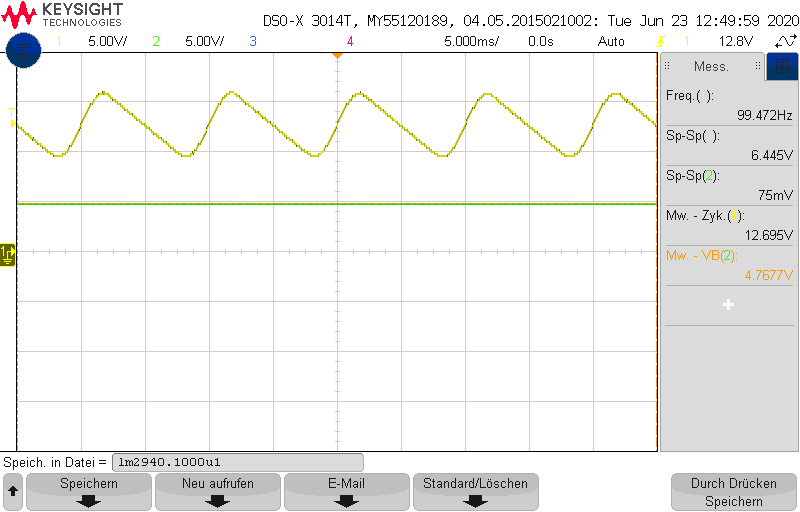
\includegraphics[width = \costumPicWidth]{Lab_5/Messungen/lm2940.1000u1.png}
    \caption{Spannungsripple LM2940, $C_1=1000\mu F$}
    \label{fig:V_rip_lm2940_1000u}
\end{figure}

\begin{figure}[H]
    \centering
    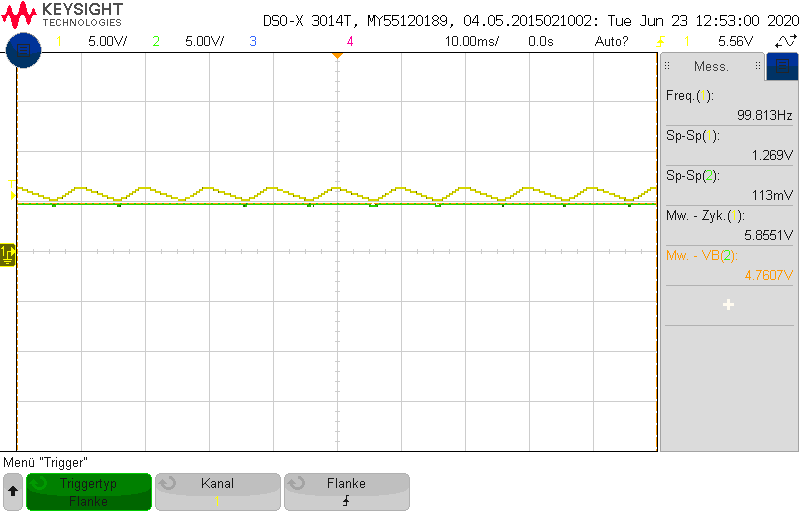
\includegraphics[width = \costumPicWidth]{Lab_5/Messungen/lm2940.min4701.png}
    \caption{Spannungsripple LM2940, $C_1=4700\mu F$}
    \label{fig:V_rip_lm2940_1000u}
\end{figure}

\begin{figure}
    \centering
    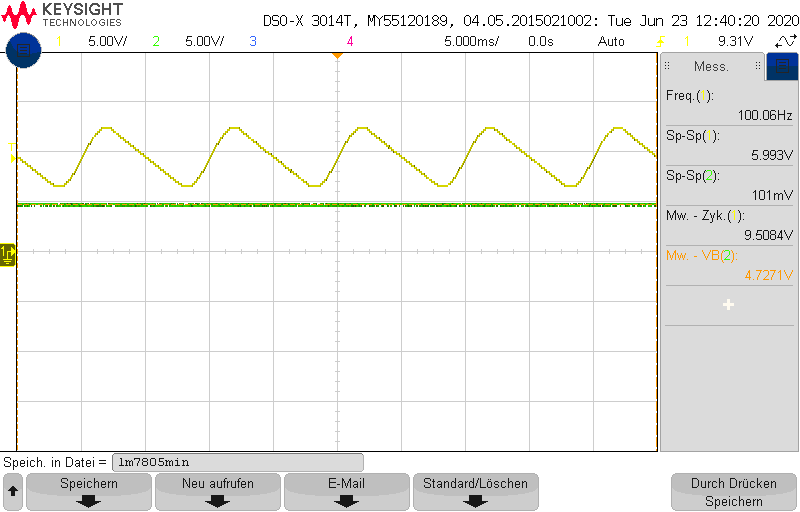
\includegraphics[width = \costumPicWidth]{Lab_5/Messungen/lm7805min.png}
    \caption{Spannungsripple LM7805, $C_1=1000\mu F$}
    \label{fig:my_label}
\end{figure}
\begin{figure}
    \centering
    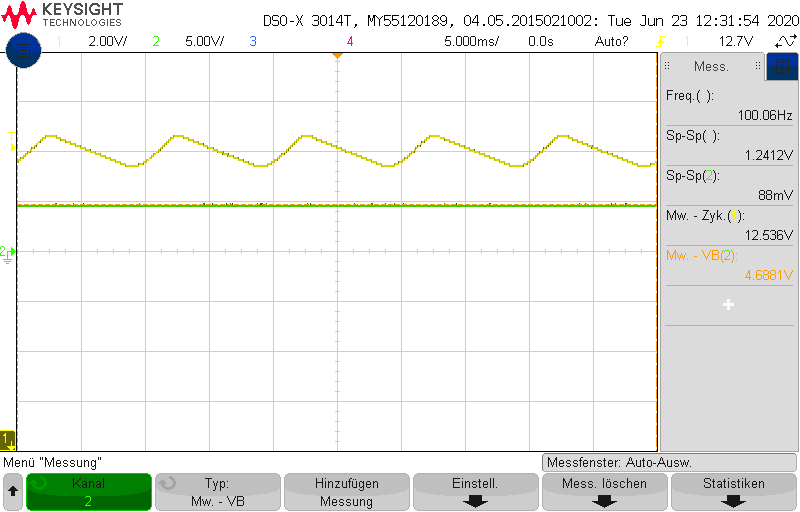
\includegraphics[width = \costumPicWidth]{Lab_5/Messungen/lm7805.4700u.png}
    \caption{Spannungsripple LM7805, $C_1=1000\mu F$}
    \label{fig:my_label}
\end{figure}
\begin{table}[H]
\centering
\caption{Messergebnisse Festspannungsregler}
\label{tab:res_Festu_reg}
\begin{tabular}{|l|l|l|l|}
\hline
\rowcolor[HTML]{9B9B9B} 
       & $V_{PP} 1000\uF$ & $V_{PP} 1000\uF$ & minimale Eingangsspannung \\ \hline
LM2940 & $6,445\V$        & $1,3367\V$       & $6,0060\V$                \\ \hline
LM7805 & $5,993\V$        & $1,194\V$        & $6,7648\V$                \\ \hline
\end{tabular}
\end{table}
Von diesen Messungen lässt sich sagen, dass der Festspannungsregler LM7805 eine weitaus höhere Dropout Spannung benötigt um den Regelbereich nicht zu verlassen. Dies führt unter anderem zu einem höheren Wirkungsgrad. Desweiteren führt eine größerer Kondensator zu höheren Wirkungsgraden, da dieser zu einer besseren Glättung der Eingangsspannung führt und somit geringere Brummspannungen auftreten

\subsection{Wirkungsgradbetrachtung der Schaltungen}
\begin{align}
    \theta = \frac{U_{out}\cdot I_{out}}{U_{in}\cdot I_{in}} \\
    \text{ mit: } I_{in} \approx I_{out} \\
    \theta = \frac{U_{out}}{U_{in}}
\end{align}